\documentclass[12pt,a4paper,twoside]{article}

% Include packages that contain additional features, for example including special mathematical characters and images in your document
\usepackage{amssymb,amsmath,graphicx}
\usepackage[hidelinks]{hyperref}
\usepackage{verbatim}
%\usepackage{pdfpages}

\title{Exercises IV}
\author{Robin Greif (Exercise 3 Francisco Aros), Lia Hankla (Exercise 2 Victor Ksoll)}
\date{Due 2018/05/11}

\begin{document}
\maketitle

% Lab
\section{Exercise 1: Numerov Algorithm for the Schroedinger Equation}

\begin{figure}[h!]
  \centering
  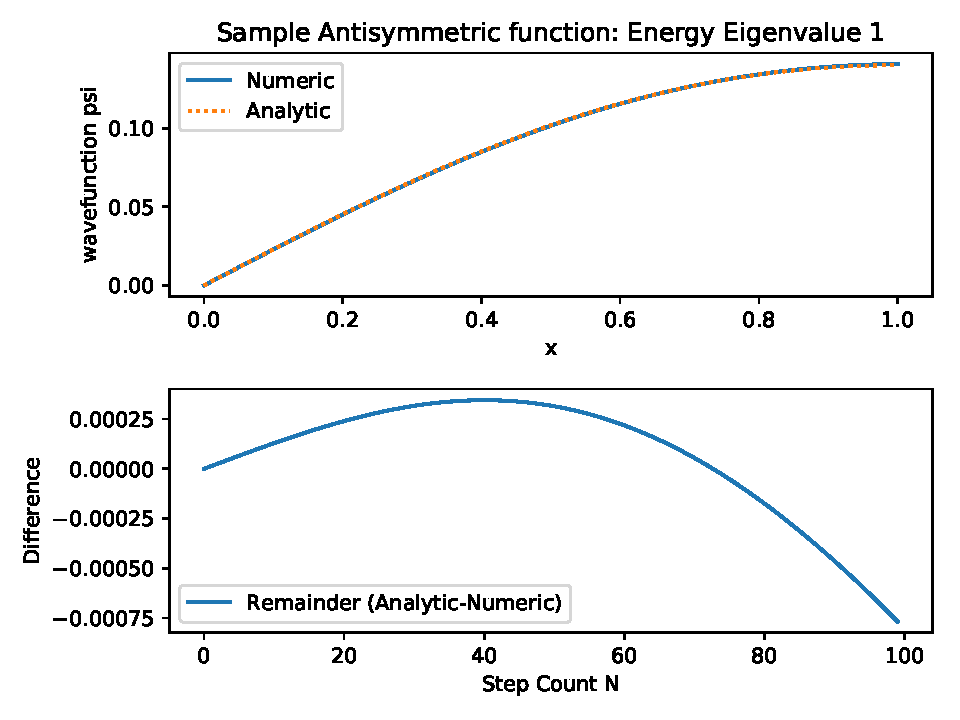
\includegraphics[width=.9\textwidth]{../exercise4_problem1_antisymEx.pdf}
  \caption{Antisymmetric solutions for harmonic oscillator using the Numerov Algorithm, compared to analytic solution} 
  \label{fig:1a}
\end{figure}

\begin{figure}[h!]
  \centering
  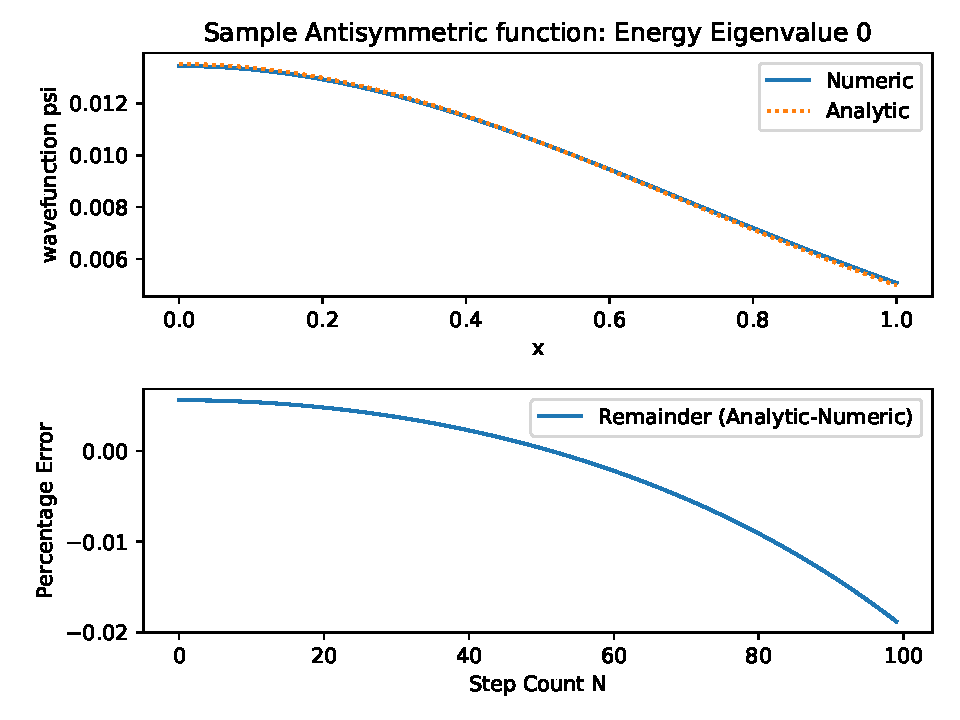
\includegraphics[width=.9\textwidth]{../exercise4_problem1_symEx.pdf}
  \caption{Symmetric solutions for harmonic oscillator using the Numerov Algorithm, compared to analytic solution} 
  \label{fig:1b}
\end{figure}


% Homework
\section*{Exercise 2: Neutrons in the grvitational field}

\begin{align*}
  0 &= \bigg(\frac{\hbar^2}{2m} \frac{\partial^2}{\partialz^2} - V(z) \bigg)
            \psi(z) + E \psi(z)  \\     
  0 &= \bigg(\frac{\hbar^2}{2m} \frac{\partial^2}{\partialz^2} - mgz \bigg)
            \psi(z) + E \psi(z)  \\     
  0 &= \bigg(\frac{\hbar^2}{2m} \frac{1}{R^2} \frac{\partial^2}{\partialz^2} - mgRx \bigg)
            \psi(x) + mgR\epsilon \psi(x)  \\       
  0 &= \psi''(x) + (\epsilon - x) \psi(x)  
  \label{eq:neutron_grav}
\end{align*}

where we used
\begin{align*}
  R &= \bigg( \frac{\hbar^2}{2m^2g} \bigg) ^(1/3)  \\
  x &= z/R  \\
  \epsilon &= \frac{E}{mgR}  
\end{align*}

with units
\begin{align*}
  [R] &= \bigg( \frac{[Energy \times time]^2}{[mass]^2 [length \times \time^{-2}]} \bigg) ^(1/3)  \\
      &= [Energy^2 \times time^4 \times mass^{-2} \times length^{-1}]  \\
      &= [[mass \times length^2 \times time^{-2}]^2 \times time^4 \times mass^{-2} \times length^{-1}]  \\
      &= [mass^2 \times length^4 \times time^{-4} \times time^4 \times mass^{-2} \times length^{-1}]  \\
      &= [length^3]  \\
  [x] &= [length]/[length^3] = [length^{-2}]  \\
  [\epsilon] &= \frac{[Energy]}{[mass][m][length \times \time^{-2}][length^3]}  \\
             &= [Energy \times mass^{-1} \times length^{-1} \times time^2 \times length^-3 ] \\
             &= [mass \times length^2 \times time^{-2} \times mass^{-1} \times length^{-1} \times time^2 \times length^{-3}]  \\
             &= [length^{-2}]
\end{align*}



\subsection*{Part 1}

\begin{figure}[h!]
  \centering
  \includegraphics[width=.9\textwidth]{../exercise4_problem2_numIntegration.pdf}
  \caption{Numerically integrating Eq.~\ref{eq:neutron_grav}}
  \label{fig:2a}
\end{figure}

\begin{figure}[h!]
  \centering
  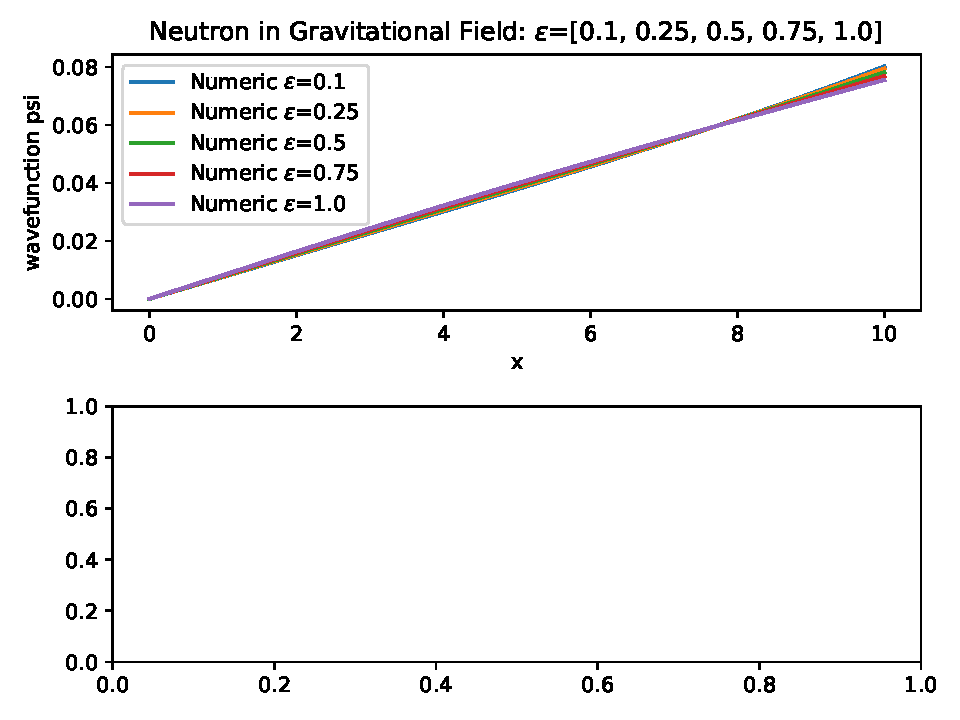
\includegraphics[width=.9\textwidth]{../exercise4_problem2_varyEps.pdf}
  \caption{Numerically integrating Eq.~\ref{eq:neutron_grav} with varying $\epsilon$}
  \label{fig:2b}
\end{figure}


\subsection*{Part 2}




%
The code for the exercises is as follows:
\verbatiminput{../exercises04.py}




\end{document}

